\section{Einleitung}\label{sec:ein}
Einleitung nach \autoref{sec:ein}

\section{Hauptteil}\label{sec:haupt}
\subsection{Bilder und Grafiken}\label{subsec:grafiken}
\subsubsection{Bilder}\label{subsubsec:bilder}
Bilder befinden sich im Image-Orgner und lassen sich mit \textbackslash image\{Breite\}\{Datei im Image-Verzeichnis\}\{Beschriftung\}\{Label\} einbinden. \image{3cm}{logo.png}{Uni-Logo}{img:uni} Die Referenzierung erfolg mittels \textbackslash autoref\{Label\}, also z.B. \autoref{img:uni}.
\subsubsection{Grafiken mit TikZ}
Grafiken im TikZ-Framework\footnote{\url{http://www.tn-home.de/TUGDD/Stuff/TikZ_final.pdf}} lassen sich mit dem Befehl \textbackslash scaletikzimage\{Datei im Image Verzeichnis\}\{Beschriftung\}\{Label\}\{Skalierungsfaktor\} einbinden. \scaletikzimage{tikz}{TikZ-Grafik}{img:tikz}{0.9}
\subsection{Tabellen}
Tabellen lassen sich mit dem Environment\\
\textbackslash begin\{longtable\}[H h t b c]\{Spaltendefinitionen\} ...\\
\qquad\qquad \textbackslash caption\{Tabellenunterschrift\}\\
\qquad\qquad \textbackslash label\{Label\}\\
\textbackslash end\{longtable\}\\
 definieren\footnote{\url{ftp://ftp.dante.de/pub/tex/macros/latex/required/tools/longtable.pdf}}\\
\begin{longtable}[H]{|p{0.2\textwidth}|p{0.2\textwidth}|p{0.2\textwidth}|}
\hline
A&B&C\\
\hline
\caption{Tabelle 1}
\label{tab:tab1}
\end{longtable}

\subsection{MCC vs MEC}
\begin{tikzpicture}
\tkzKiviatDiagram[scale=1.25,label distance=.5cm,
        radial  = 5,
        gap     = 1,  
        lattice = 5]{Distance To UE,Latency,Jitter,Computational Power,Storage Capacity}
\tkzKiviatLine[thick,color=blue,mark=none,
               fill=blue!20,opacity=.5](10,10,10,8,8)
\tkzKiviatLine[thick,color=darkgray,
               fill=green!20,opacity=.5](2,2,2,4,4) 
\tkzKiviatGrad[prefix=,unity=100,suffix=\ \texteuro](1)  
\end{tikzpicture}

\subsection{Code-Ausschnitte}
Pseudo-Code Ausschnitte lassen sich mit \textbackslash pseudo\{Name des Algorithmus\}\{Label\}\{Datei im Code-Verzeichnis\} einbinden.
\pseudo{Mittelwert}{lst:mean}{code}
\section{Zitate}
Mit \textbackslash nocite*\{\} lassen sich alle Einträge in der Bibliography ausgeben. Mit \textbackslash cite[S. xx]\{Key\} lassen sich Zitate einfügen. Z.B. \cite[S. 234]{Kurose12} \nocite*{}
\subsection{Abkürzungen}

Abkürzungen können mit \textbackslash nomenclature\{Abk\}\{\textbackslash m\{Abk\}ürzung\} \nomenclature{Abk}{\m{Abk}ürzung} angegeben werden. Diese werden alphabetisch sortiert in ein Abkürzungsverzeichnis aufgenommen.

